\chapter{Introduction}

This document is the Software Specification Requirements (SRS) of the website, afetbilgi.com, developed by a group of METU students and graduates after the Pazarcik Earthquake on February 6, 2023.

\section{Purpose of the System}

Afetbilgi.com is a website that tries to deliver accurate information to people.
After the Pazarcik Earthquake, there was a lot of misinformation on social media platforms, and the infrastructure quality in the earthquake zone was terrible. 
Therefore people who needed help were having trouble finding the correct information.
Thanks to afetbilgi.com, it delivers the correct information with accuracy, speed, and simplicity principles.

\section{Scope}

The website is named afetbilgi.com, and the users will be able to reach important telephone numbers and locations in a disaster situation. \\
The scope of the system can be listed as \\
\begin{itemize}
    \item The system provides users with essential locations as a map view, and users can filter the places such as hospitals, food delivery places, and temporary accommodation locations. When selected, it is navigated using the google maps navigation system.
    \item The system provides users the valid active hospitals, evacuation points, safe gathering places, and temporary accommodation places in the disaster area to download as a pdf format. Moreover, in the file for all locations, they validate whether the information is correct and google maps navigation links.
    \item The system provides users to select the city where they live so that it filters the information accordingly.
    \item The system provides users with valid solidarity campaigns, monetary donation links, and blood and stems cell donation places. 
\end{itemize}

\section{System Overview}

This section of the document will provide detailed information about the system with its components. 

\subsection{System Perspective}

The purpose of the development of afetbilgi.com is mainly to help people who are affected by disasters like earthquakes.
For this purpose, the website can be used by all people, not just limited to people in a disaster area. 
People who are affected can use this application to get any sort of help.
The other people can find helpful links or locations to help people who are in need. 
Thanks to this application, a general mobilization can be achieved within the region; therefore, the reach of aid can be accelerated, and a wider environment can be easily reached.
\begin{figure}[H]
    \begin{center}
        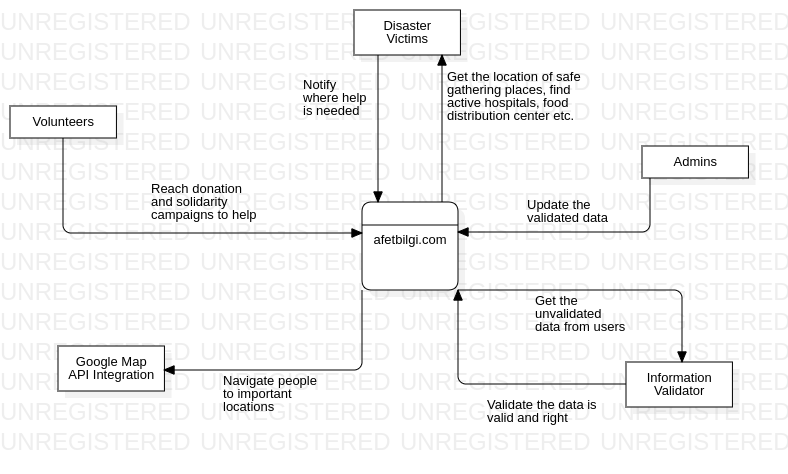
\includegraphics[scale = 0.60]{assets/SystemContextDiagram.png}
        \caption[System Context Diagram]{System Context Diagram for afetbilgi.com}
    \end{center}
\end{figure}

\subsubsection{System Interfaces}

\begin{itemize}
    \item \textbf{Google Maps API: } Afetbilgi.com uses Google Maps API to navigate people to locations that are on the website to the user. This system shows users where they are, close evacuation points, emergency gathering areas, temporary accommodation places, food distribution centers, gas stations, active hospitals, and pharmacies. With this integration, in emergency cases, people can find where and how to go rapidly. Thus, it may increase the survival rate in vital situations. 
    \item \textbf{Database Management Interfaces: } Authorized persons validate the pieces of information in teams. Afetbilgi.com admins update the database with the validated information thanks to the validation teams and volunteers. With this mobilization, this system works with accuracy, speed, and simplicity principles. It also prevents disinformation. In addition to that, by the city filtering system, users can reach only the needed information in emergencies. 
    \item \textbf{PDF Integration: } This system allows users to download the crucial information for the city they need since the communication and network systems may get damaged and not reachable. Therefore, downloading only the essential information may increase the speed of help.
    \item \textbf{Multi Language Support: } This system allows afetbilgi.com to reach a broader effect on the disaster situation. Foreigners in the area can reach the system more quickly.
\end{itemize}

\subsubsection{User Interfaces}

Users can use this application by using their internet browsers. When they reach the website, users can see that one of the features of the website is simplicity. All the submenus and filters are clear and straightforward. The backend and frontend of the website are lightweight; therefore, in a disaster area, users can reach the website with slow internet speeds.

\begin{figure}[H]
    \begin{center}
        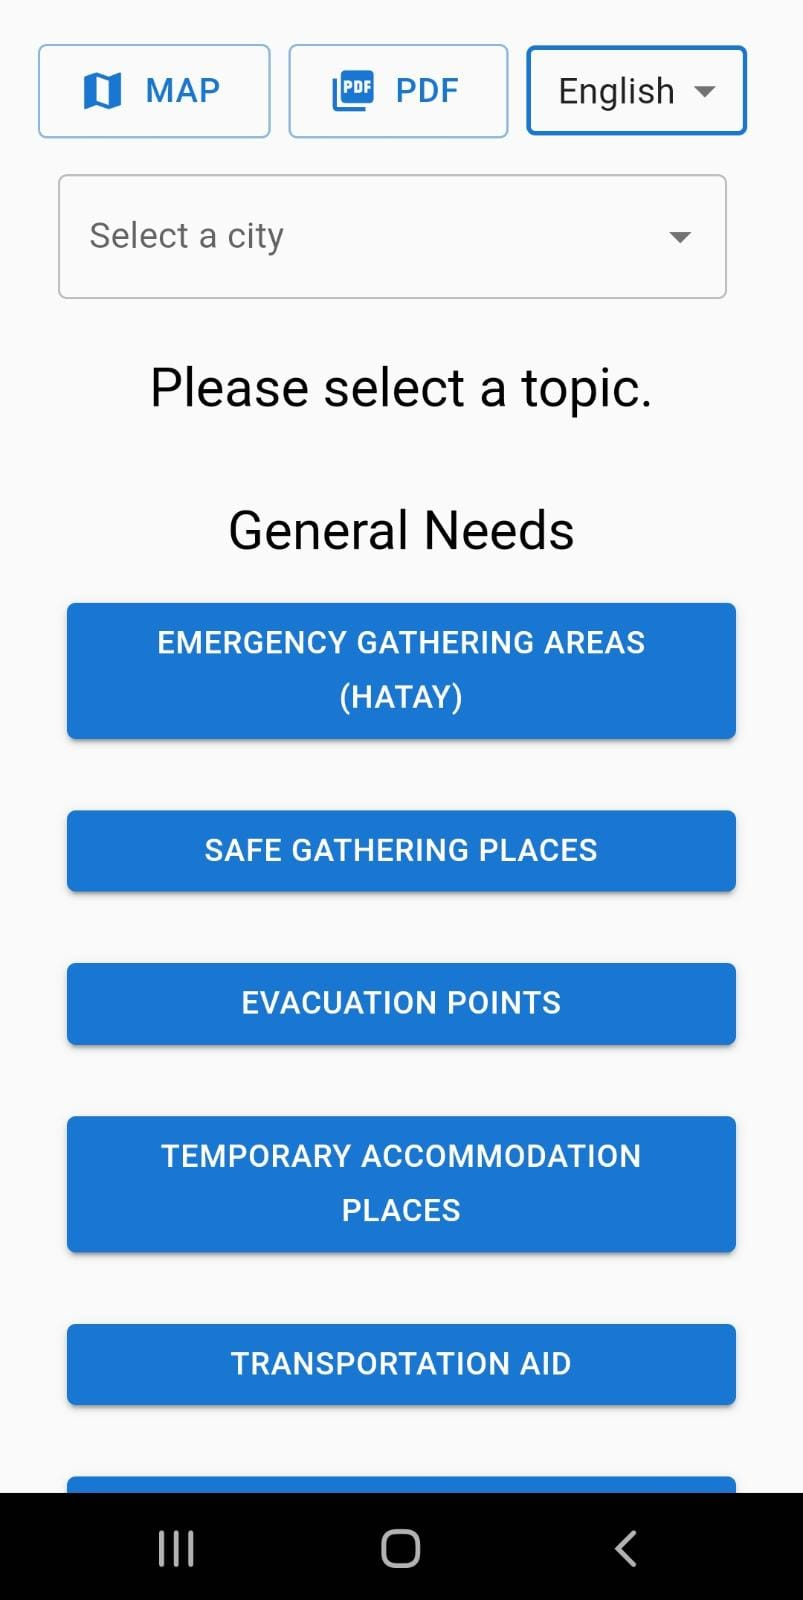
\includegraphics[scale = 0.10]{assets/mainmenu.jpeg}
        \caption[Main Menu in Mobile Devices]{Main Menu in Mobile Devices of afetbilgi.com}
    \end{center}
\end{figure}

\begin{figure}[H]
    \begin{center}
        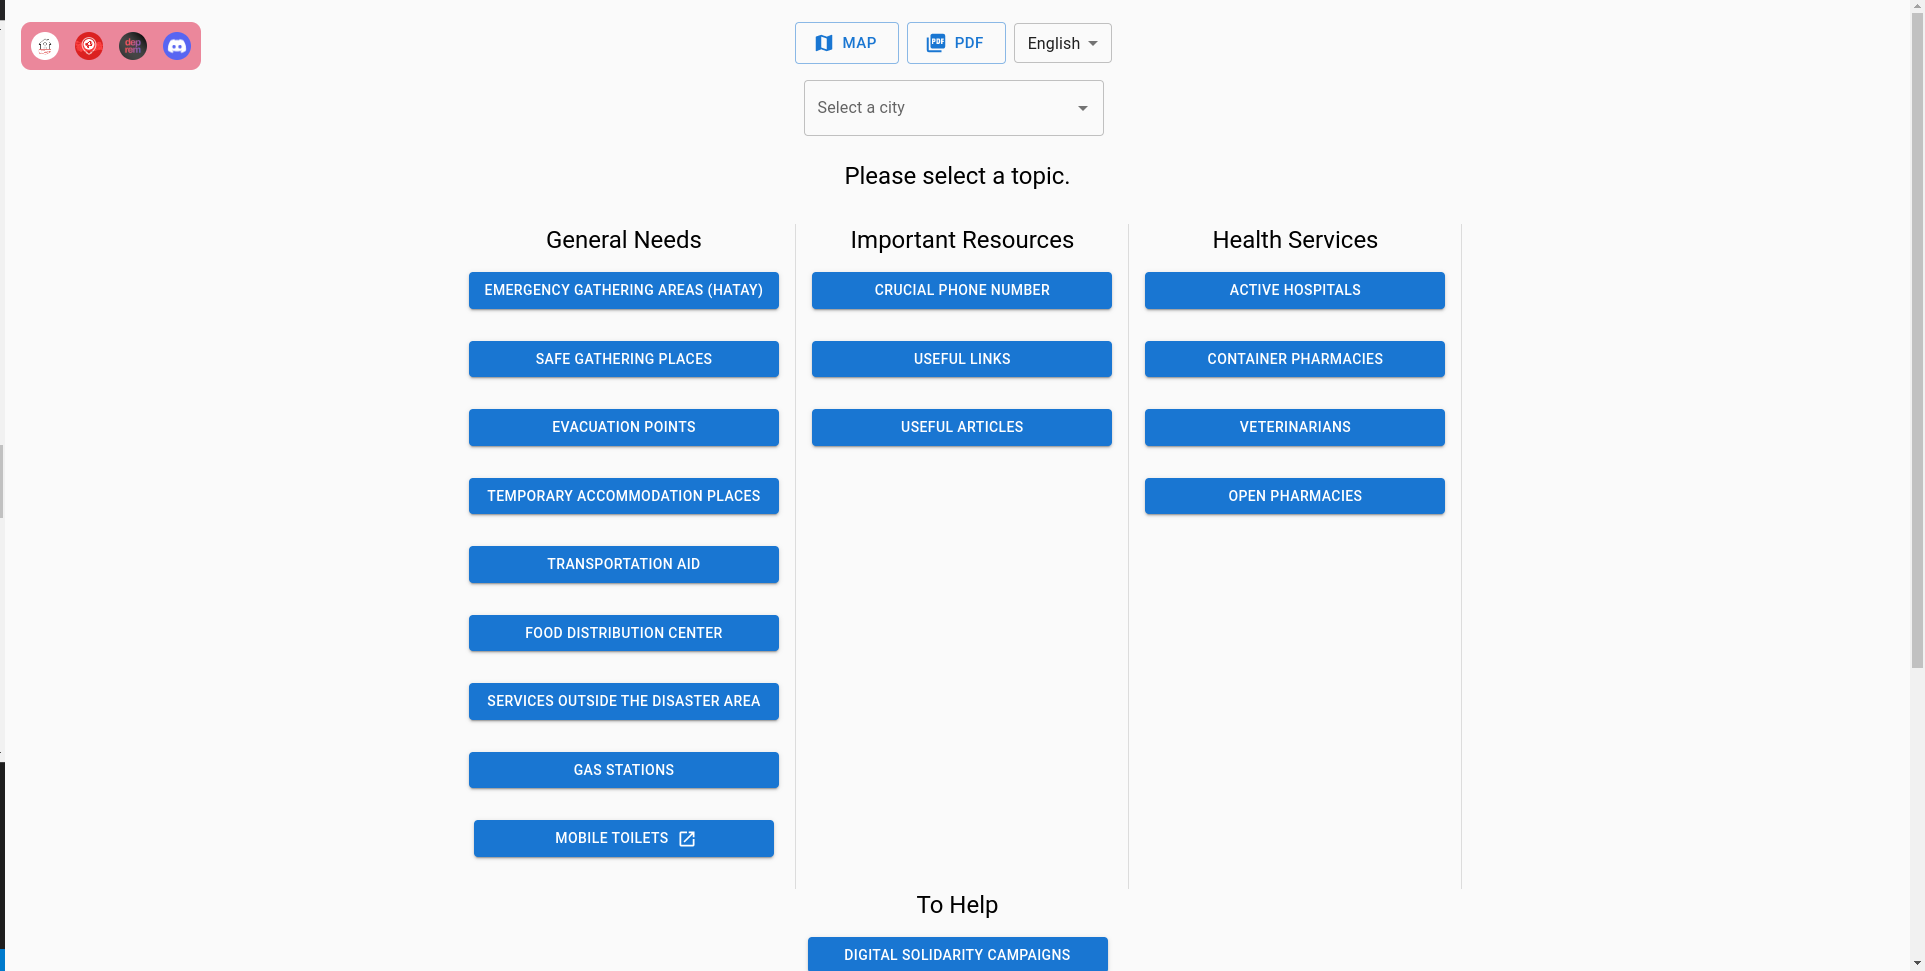
\includegraphics[scale = 0.18]{assets/desktopInterface.png}
        \caption[Main Menu in Desktop]{Main Menu in Desktop of afetbilgi.com}
    \end{center}
\end{figure}

With the Google Maps API integration, users can see their exact locations. In addition to that, they will find essential locations which they are close to them. Also, the filtering setting increases the practicality and becomes task-oriented. When the user selects the desired locations, the website redirects them to the google maps navigation system. 

\begin{figure}[H]
    \begin{center}
        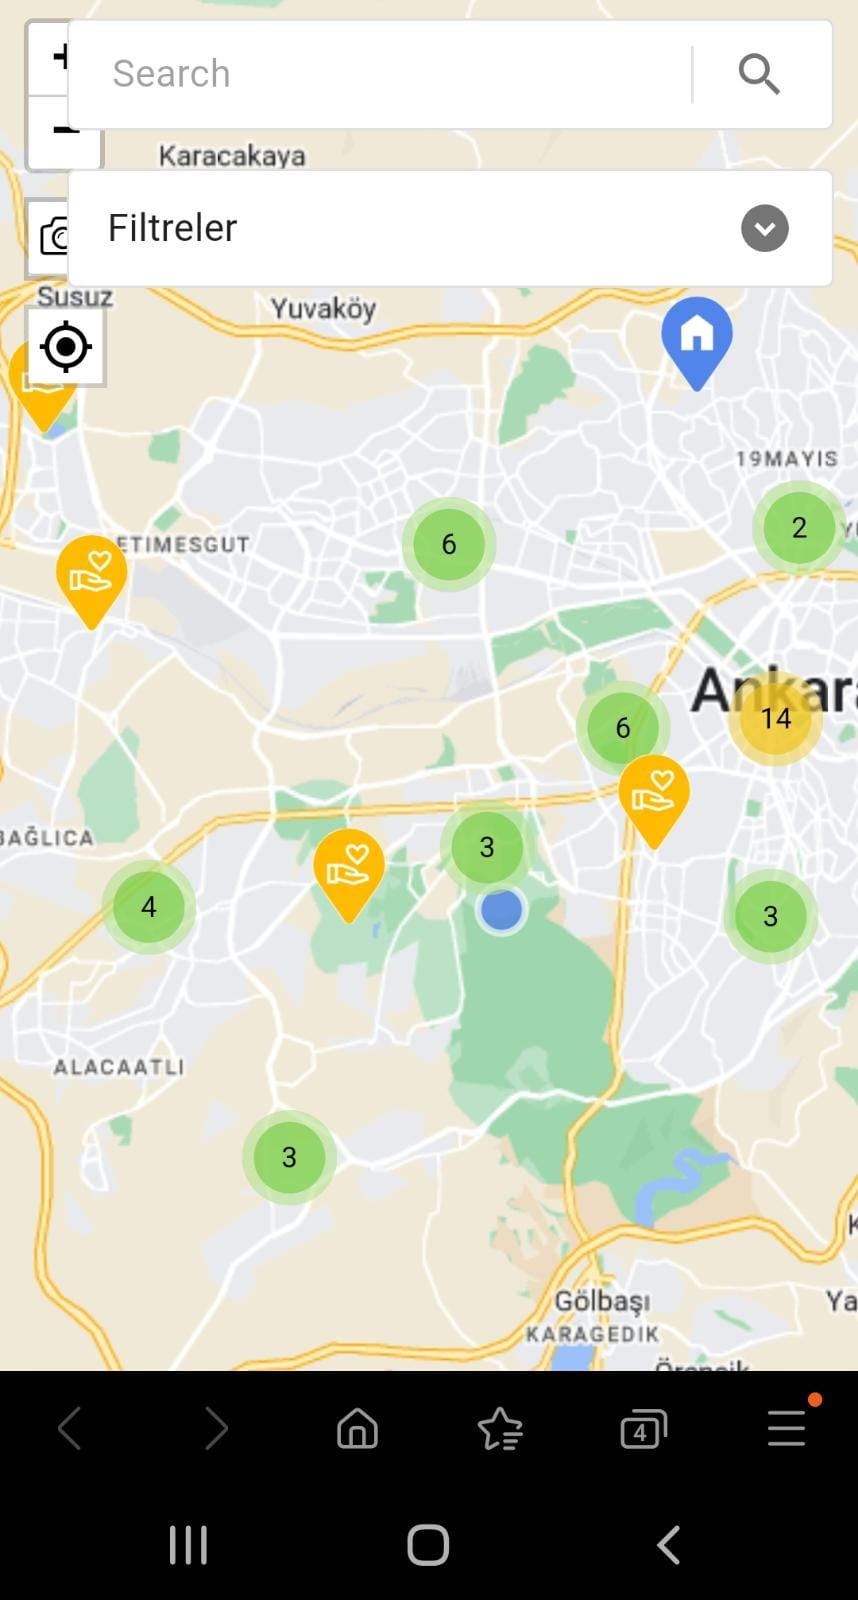
\includegraphics[scale = 0.15]{assets/maps.jpeg}
        \caption[Maps Integraion]{Maps Integration}
    \end{center}
\end{figure}

\begin{figure}[H]
    \begin{center}
        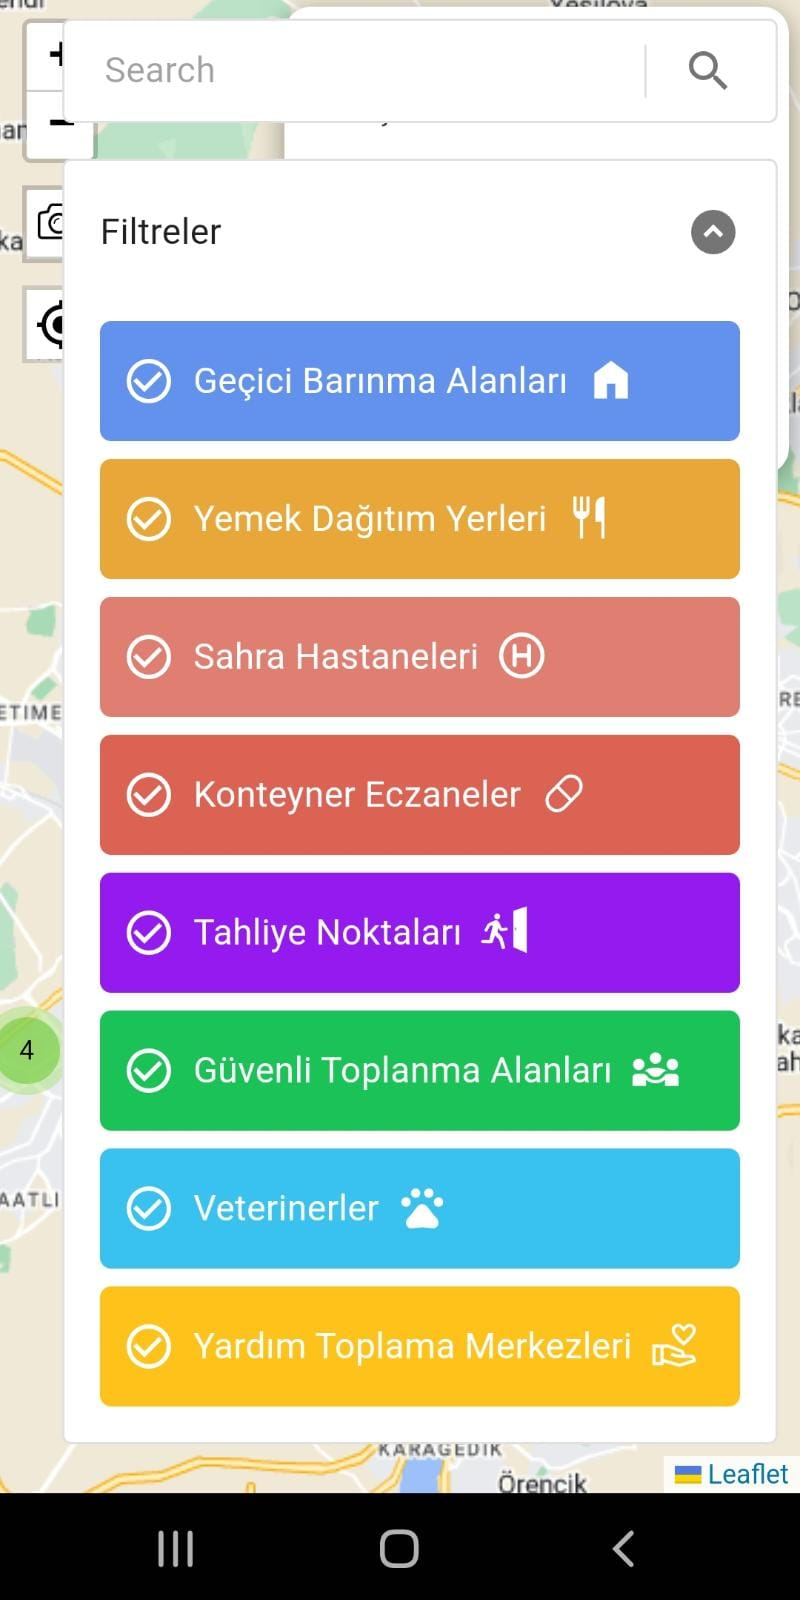
\includegraphics[scale = 0.15]{assets/filter.jpeg}
        \caption[Filter Settings for Map]{Filter Settings for Map}
    \end{center}
\end{figure}

Users can download all the information by selecting the specific cities or all cities in PDF format to access the information more quickly in a disaster situation. The application was developed for the Pazarcik Earthquake, and the system shows the cities affected by these earthquakes.

~\par There is a lot of different submenu in the application. These menus are under the subtopics, which are general needs, essential resources, health services, and to-help topics. Some of these submenus can be seen in Figure 1.7 and Figure 1.8. According to the information users search, it lists the desired information on the screen. Also, it allows filtering like the other functions. 

\begin{figure}[H]
    \begin{center}
        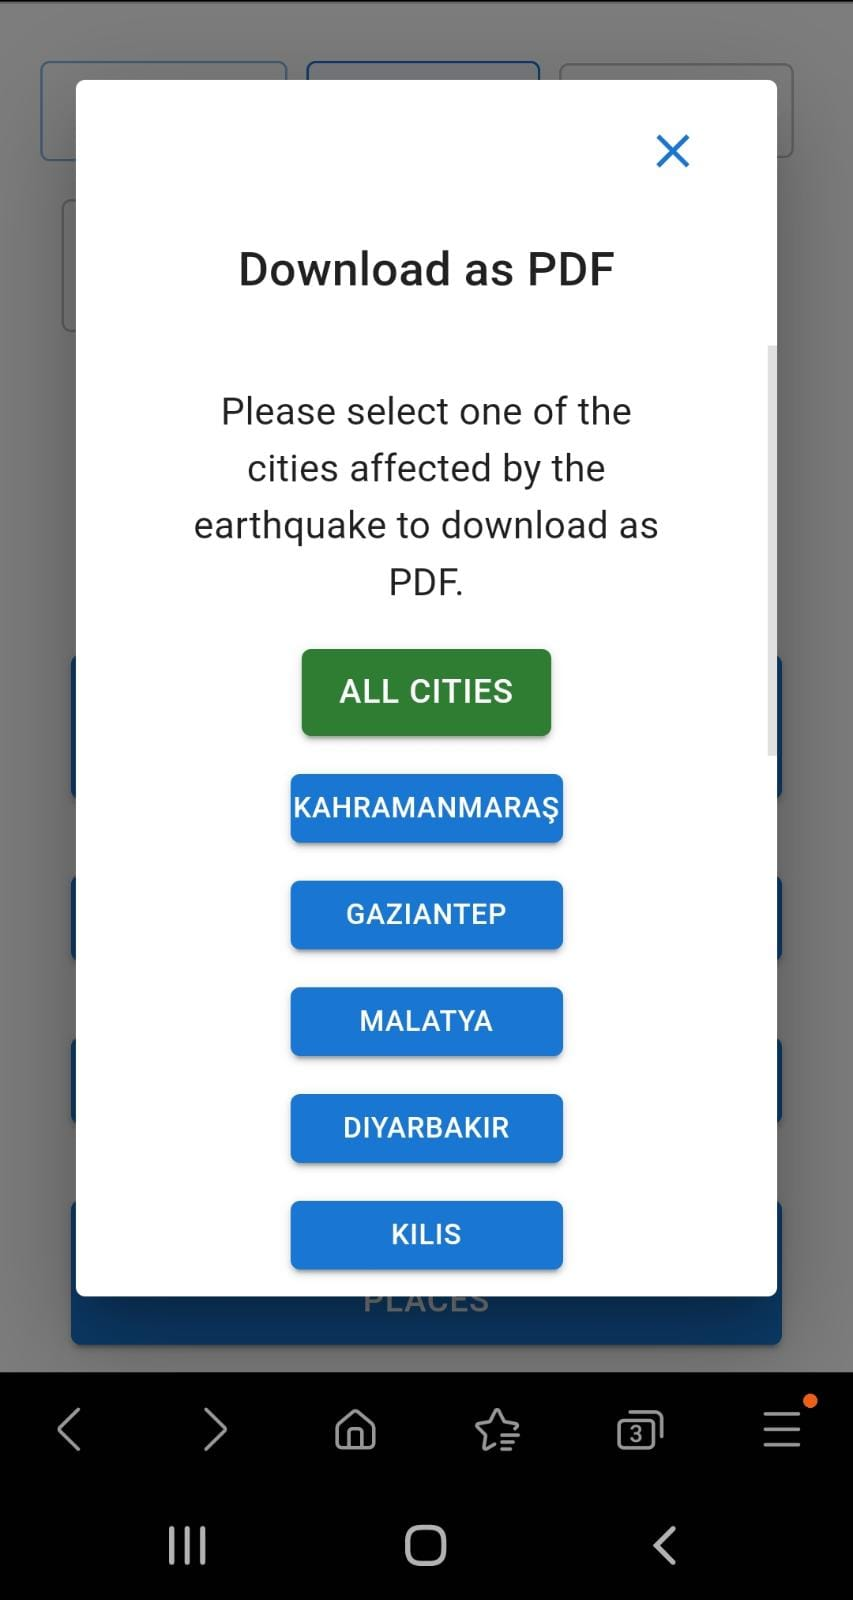
\includegraphics[scale = 0.15]{assets/pdf.jpeg}
        \caption[PDF Download Menu]{PDF Download Menu by Selecting Cities}
    \end{center}
\end{figure}


\begin{figure}[H]
    \begin{center}
        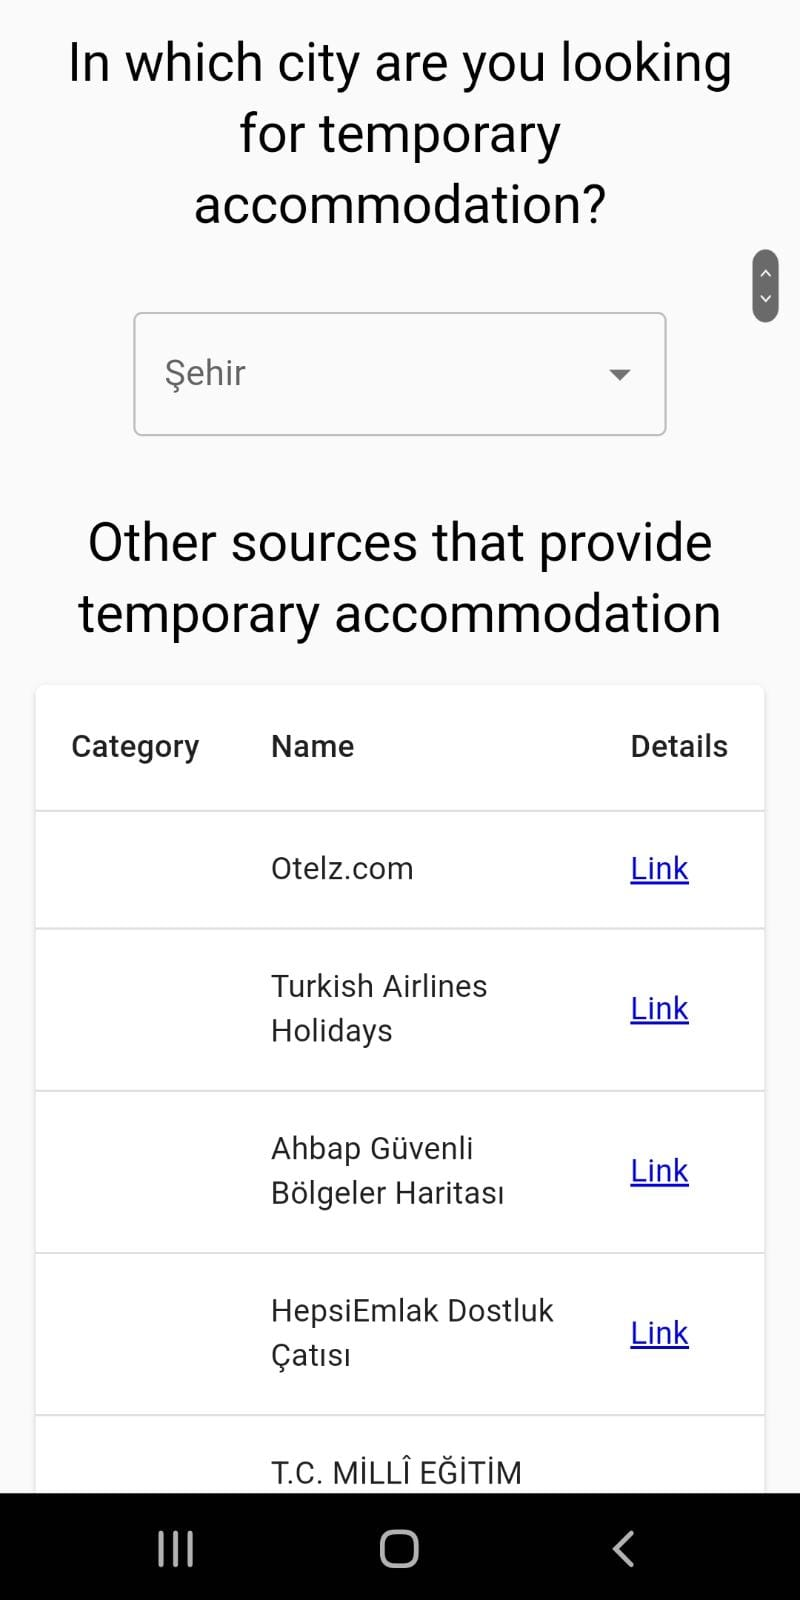
\includegraphics[scale = 0.15]{assets/accommodation.jpeg}
        \caption[Accommodation Menu]{Accommodation Menu}
    \end{center}
\end{figure}

\begin{figure}[H]
    \begin{center}
        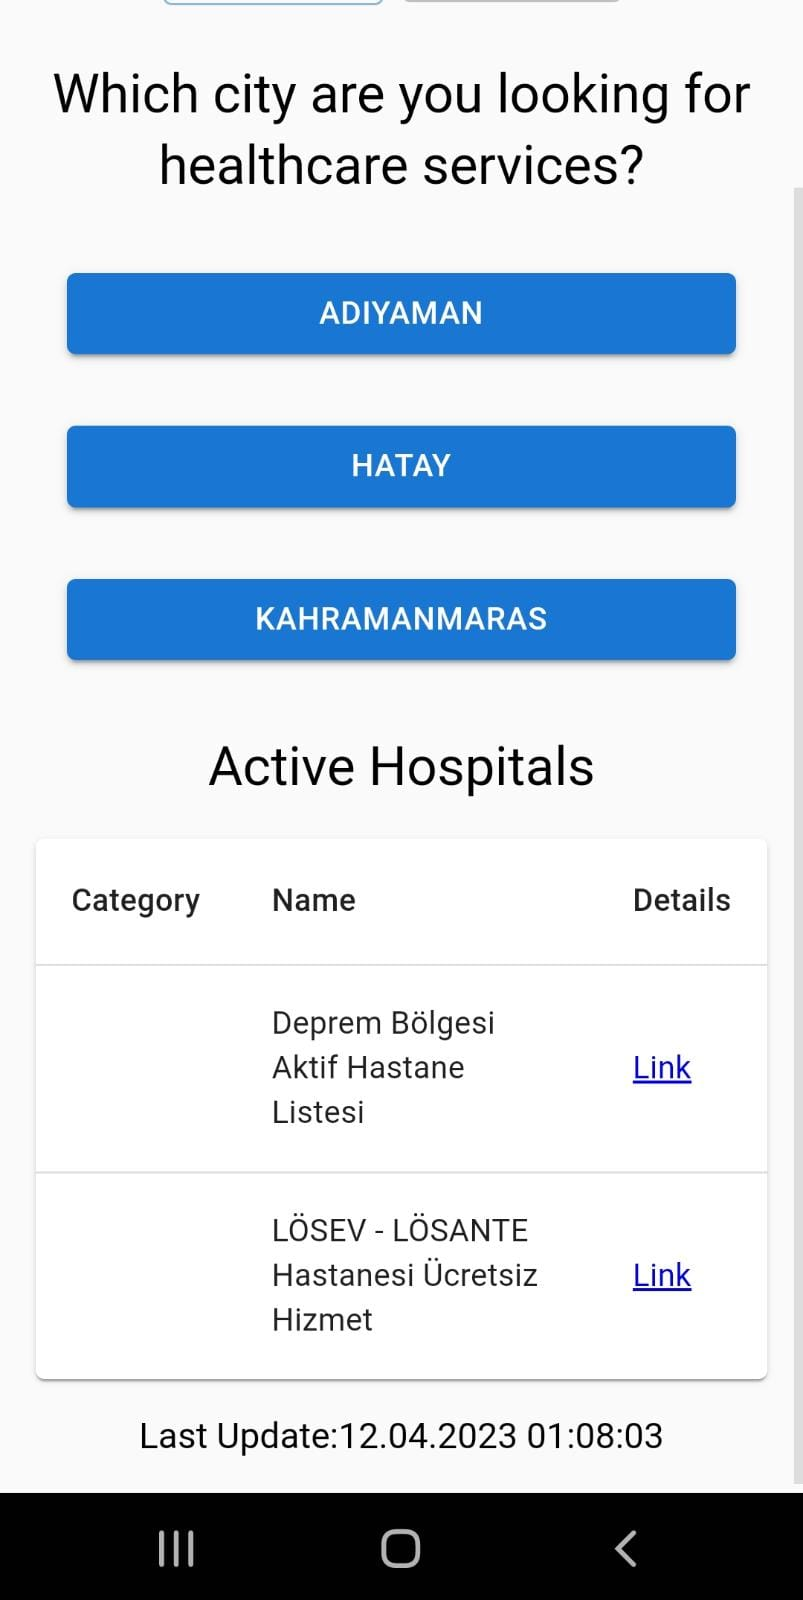
\includegraphics[scale = 0.15]{assets/healthcareinterface.jpeg}
        \caption[Healthcare Services Menu]{Healthcare Services Menu}
    \end{center}
\end{figure}

\subsubsection{Hardware Interfaces}

The system requires a device that has internet access. If the user wants to use Google Maps API, it should also have a GPS on its device.

\subsubsection{Software Interfaces}

\begin{itemize}
    \item \textbf{Database: } The system uses JSON files to store the data. This system does not require a complicated database system.
    \item \textbf{Operating Systems: } The system can be reachable by any device which has an internet browser and access.
    \item \textbf{Google Maps: } The system uses Google Maps to show the essential locations and where the user is on the map and allow them to reach them.
\end{itemize}

\subsubsection{Memory Constraints}

There is no issue with memory constraints in the system. The system should have enough memory to hold necessary information; however, it requires a very low memory which can be sustainable easily. 

\subsubsection{Operations}

The operations provided by afetbilgi.com can be partitioned into: \\

\textbf{User operations: }

\begin{itemize}
    \item Reaching important resources
    \item Seeing Location of Healthcare Services
    \item Reaching other websites to help victims
    \item Seeing contact info and location places associated with general needings
    \item Filters the info by cities
    \item Seeing data of website on a Map
    \item Contacting with Developers and Maintainters
\end{itemize}

\textbf{Admin operations: }
\begin{itemize}
    \item Validate the information
    \item Update the information
\end{itemize}

\textbf{System Operations: }
\begin{itemize}
    \item Creating a PDF document which includes info
    \item Multi Language Support
\end{itemize}

All details of these operations will be explained in Functions Section (3.2).

\subsection{System Functions}

\subsection{Stakeholder Characteristics}

\subsection{Limitations}

\section{Definitions}